\chapter{Introduction\label{cha:introduction}}
%% \ifdraft only shows the text in the first argument if you are in draft mode.
%% These directions will disappear in other modes.
\ifdraft{State the objectives of the exercise. Ask yourself:
  \underline{Why} did I design/create the item? What did I aim to
  achieve? What is the problem I am trying to solve?  How is my
  solution interesting or novel?}{}

Keflavík International Airport (IATA:KEF, ICAO:BIKF) is the major gateway to Iceland currently with two functioning runways. 
There has been a gradual increase of passengers travelling through Keflavik Airport in the recent years with over eight million passengers and 62,3 thousand air transport movements in 2017 \cite{isavia_facts_2017}. For 2018 the passenger numbers show a growth of 13.1\% on average (at the time of writing) from the previous year \cite{isavia_pass_statistics_2018}. The increase in traffic at Keflavík Airport can encounter constrained capacity of the runway during peak traffic periods. 
A significant constraint of this process is caused by separation regulations of aircraft due to wake-vortices. These are specified by rules established by the European Aviation Safety Agency (EASA)  for each type of aircraft based primarily on the weight of the aircraft. The general flight safety requirements are established by the International Civil Aviation Organisation (ICAO) for maintaining safe distance between aircraft

\section{Background and Literature Review}

%\ifdraft{Provide background about the subject matter (e.g. %How was morse code developed?  How is it used today?). 
%This is a place where there are usually many citations.
%It is suspicious when there is not.
%Include the purpose of the different equipment and your %design intent. 
%Include references to relevant scientific/technical work and %books.
%What other examples of similar designs exist?
%How is your approach distinctive?

%If you have specifications or related standards, these %mustscribed and cited also.  As an example, you might cite %the specific
%RoboSub competition website (and documents) if working on the %lighting system for an AUV

%%% Glossary is broken, do not use --foley
%% \gls{auv}\footnote{Autonomous Undersea Vehicle}.
%
%% Notice that there is now information on the AUV in the %Index %and Acronyms.
%% It isn't in the \gls{glossary} because we didn't put it %there.
%\index{AUV}
%}{}



\subsection{Current understandings of wake vortex behaviour}
The wing of an aircraft can be regarded as a beam of finite length with aerofoil as cross section \cite{hansen2015aerodynamics}\fxnote{Find a more appropriate source for citation or drop it if unnecessary. Read about induced vertical flow in a book on aerodynamics}.
The lift effect is created by the differential pressure between the lower and the upper side of the wing. At the wing tips the high pressure flow from the lower side leaks around the tip and to the upper side of the wing. Thus the streamlines over the wing are pushed inwards, while the streamlines under the wing are pushed outwards. A finite lifting wing leaves behind a continuous sheet of stream-wise vorticity  \cite{hansen2015aerodynamics}\fxnote{Find a more appropriate source for citation }.  This manifests itself in multiple trailing swirls of the airflow that mix together and roll up into two main counter-rotating vortices aft of the wing as illustrated in Figure \ref{fig:vortex_develop} \cite{magazine_aibus_safety, Breitsamter2011Feb, gerz_commercial_2002}. Between the vortices the air moves downwards while outside the induced flow is upwards. Those vortices are also known as wake turbulence. 
The kinetic energy contained in the vortices is dependent on the weight and aerodynamics of the generating aircraft. The cross flow velocities in the core region of the trailing vortices can reach $360$ km/h and the vortices can stay effective up to hundred wing spans. This can result in wake vortices lasting for several minutes and up to $30$ km behind larger aircraft \cite{Breitsamter2011Feb, gerz_commercial_2002}. 

\begin{figure}
    \centering
    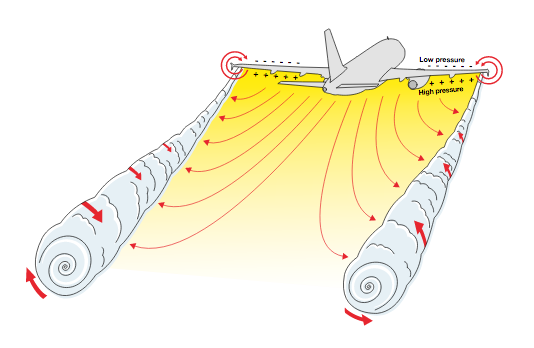
\includegraphics[width=0.8\textwidth]{graphics/WakeVortexPlane.png}
    \caption[Wake vortex roll-up process]{Wing vortex evolution and roll-up process. Two main vortices form behind the aircraft turning in opposite directions, clockwise behind the left wing (seen from behind) and anti-clockwise behind the right one \cite[p. 043]{magazine_aibus_safety}} \label{fig:vortex_develop}
\end{figure}

\subsection{Ground effect and decay process}

Near ground on approach the wake vortices tend to descend slowly to an altitude of about one half of the initial separation.
Upon reaching this point the descent will stop and then ascend slowly. This "re-bounce" effect is caused by the presence of the ground and carries with it the formation of a second pair of induced vortices outside and bellow the main vortex. 
In the presence of stable cross-wind conditions the decay of the downwind vortex is not identical to the upwind vortex and the descent rate may vary significantly \cite{Hallock2018Apr}. 
The trajectories of the vortex pair may be modified and the upwind vortex could stall over the runway while the downwind vortex ascends and decays faster (Figure \ref{fig:vortex_ground_effect}).
Measurements have shown that the lateral/sideways motion of a vortex in an airport environment could range between $229$ m and $518$ m and in some cases even $762$ m, which is the basis for the "2500-foot"  rule separation in parallel runways configuration \cite{Hallock2018Apr, hallock2004summary, hallock2003wake}. The vertical descent rate of vortices for medium commercial aircraft in stable atmosphere  is shown to be around $1.5-2.5$ m/s for the first $30$ s after which the descent slows and eventually approaches zero at $152-274$ m below the flight path, and for heavier aircraft decaying vortices have been observed at $305$ m and below of the flight path  \cite{lissaman1973aircraft, Hallock2018Apr}. 
Aerodynamic properties of the aircraft govern the vortex roll-up process and ambient atmospheric conditions dominate the behaviour of the vortices forcing instability and eventual decay of the vortices \cite{Hallock2018Apr}.
Several factors that drive the decay rate of the vortex pair have been formulated:
\begin{itemize}
    \item Atmospheric turbulence extracts energy from the vortex and reduces its strength leading to a faster wake decay \cite{Hallock2018Apr}.
    \item Viscosity of the atmosphere also draws out energy from the vortex but at a slower rate than the atmospheric turbulence \cite{Hallock2018Apr}.\fxnote{This needs to be explained (Ármann)}
    \item Buoyancy force acts on the vortex in a thermally stable stratified environment as a result of the lesser air density inside the vortex system and may causes stall or rebound to the flight level \cite{Holzapfel2001Feb, gerz_commercial_2002}.
    \item Vortex instability in the form of long wave sinusoidal fluctuations of the vortex core (Crow instability) may occur due to light turbulence in the atmosphere and may cause the vortices to link and decay faster \cite{Hallock2018Apr, crow2003stability}.
    \item Secondary vorticity structures, vertical rib-like counter rotating flow formations may appear between the vortex pair and eventually wrap around the main vortices, leading to turbulence build inside the system and rapid circulation decay\cite{Holzapfel2001Feb, Holzapfel2003Jun}.
\end{itemize}


\begin{figure}
    \centering
    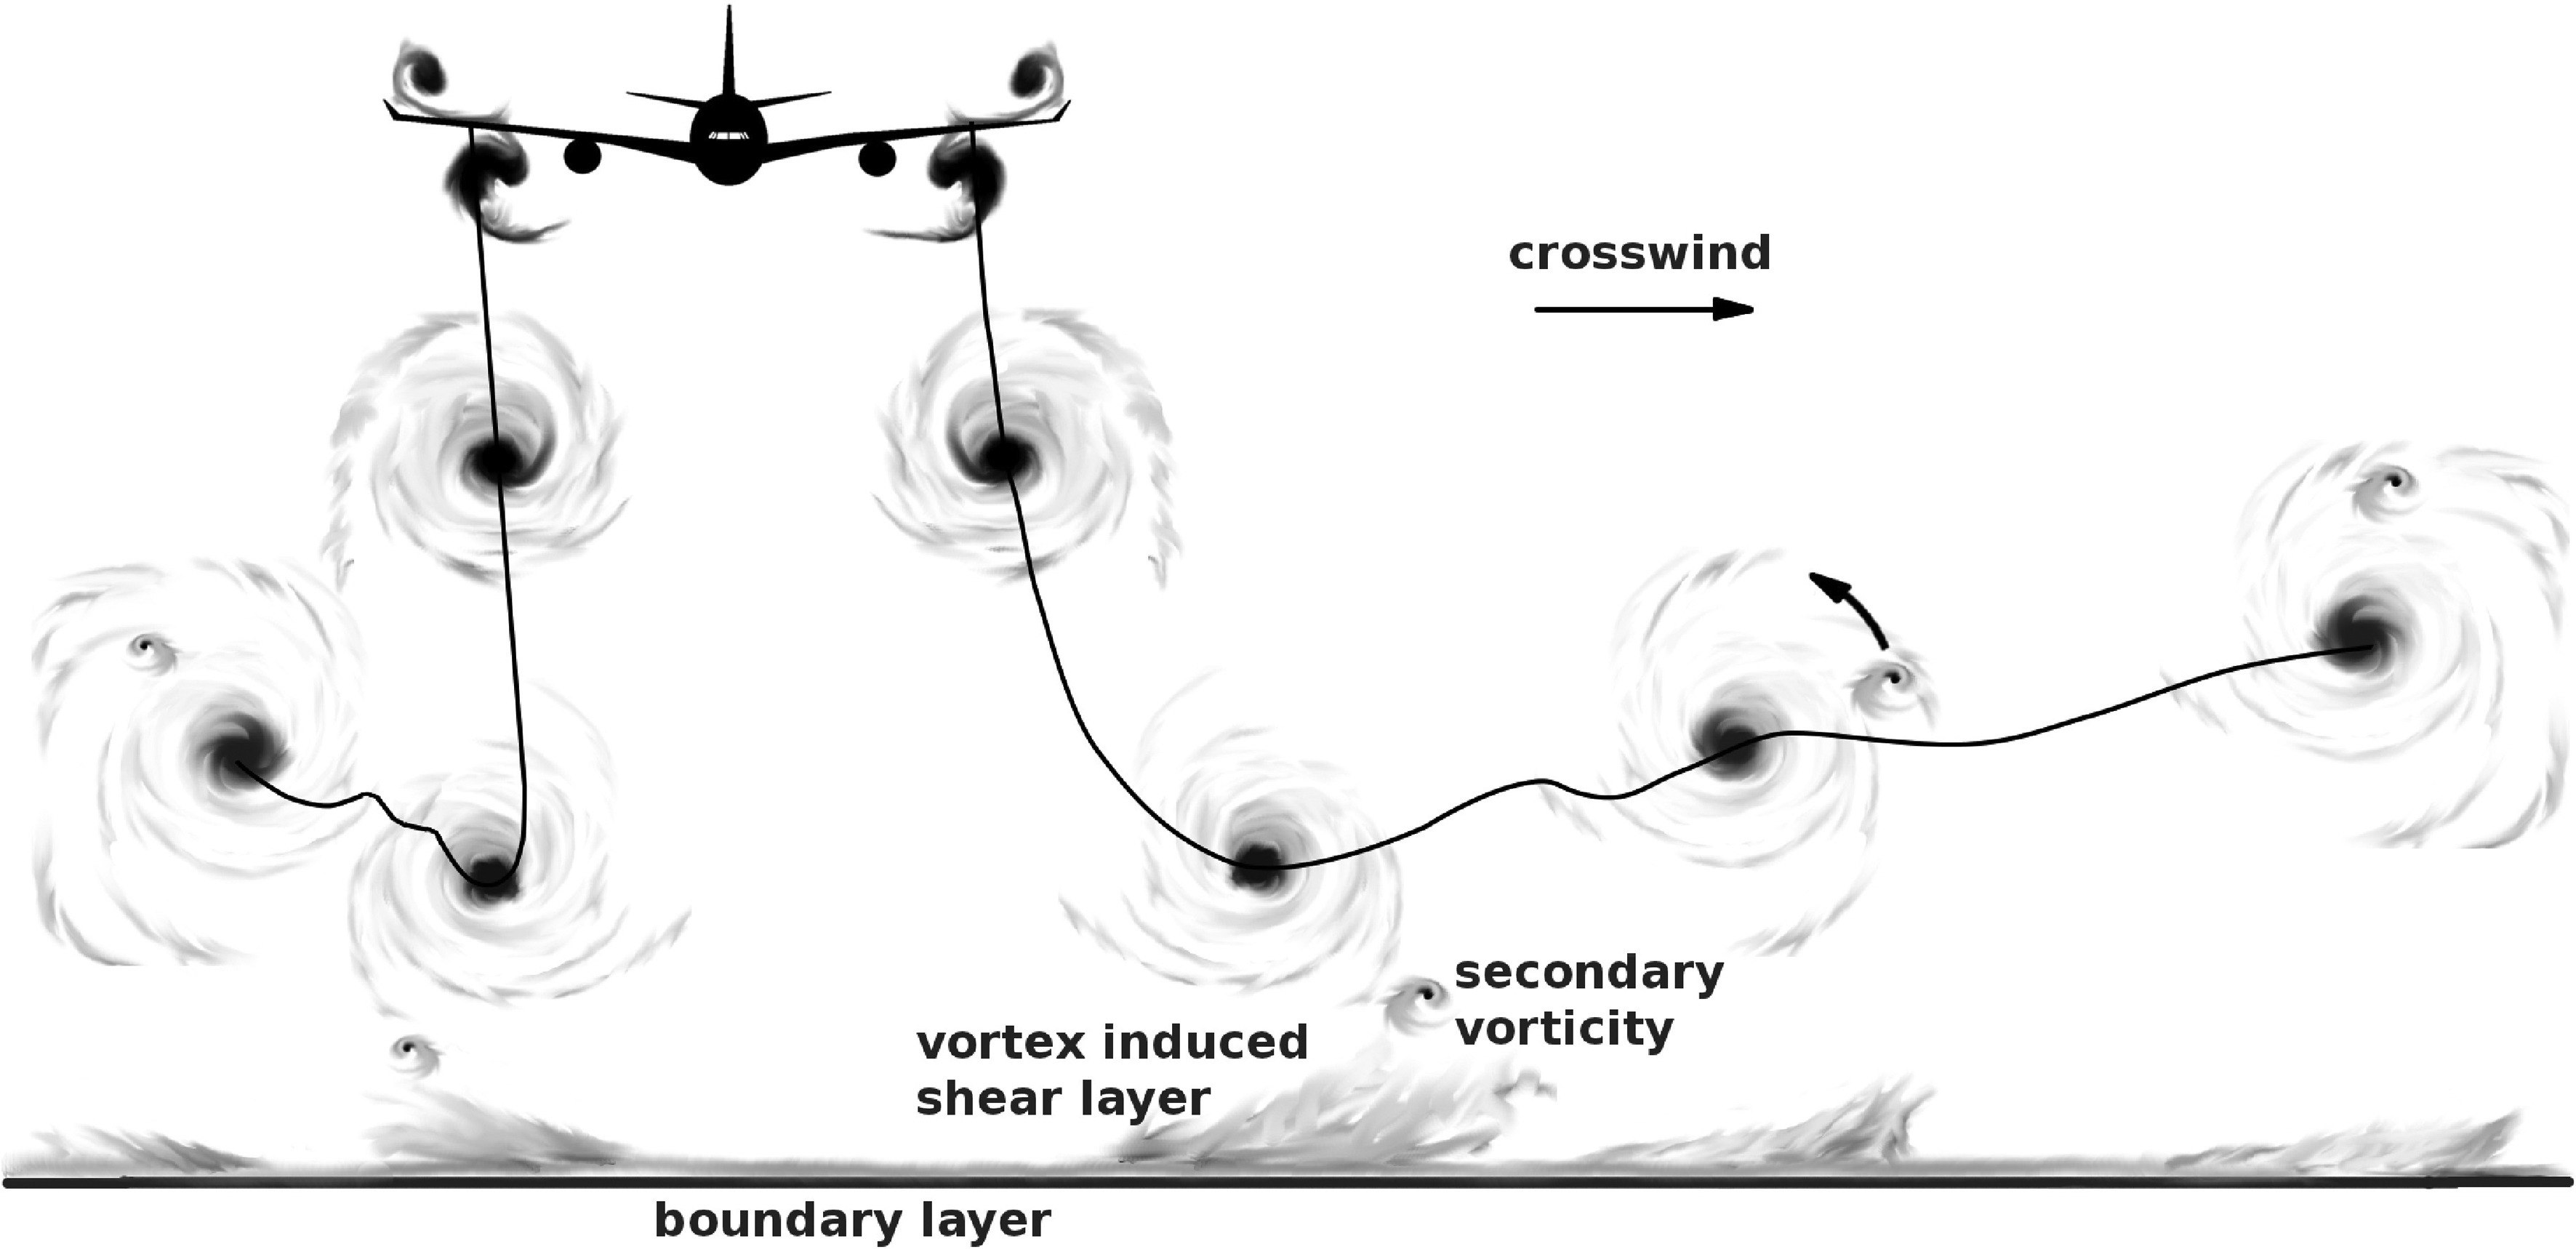
\includegraphics[width=0.8\textwidth]{graphics/Hallock_vortex_evolution.jpg}
    \caption[Wake vortex and ground effect]{Vortex evolution and ground effect \cite[p. 29]{Hallock2018Apr}.} \label{fig:vortex_ground_effect}
\end{figure}


\subsection{Wake vortex separation}
An aircraft affected by the wake vortex can experience loss of lift or an induced rolling moment and velocity fluctuations (Figure \ref{fig:vortex_encounter}).
This can lead to the up-set and potentially loss of control of an aircraft following the flight path of a preceding aircraft.
To diminish the effect of such vortices the trailing aircraft must be maintained at a safe distance behind the lead aircraft as the vortices spread laterally to either side of the flight path and are dissipated \cite{Breitsamter2011Feb}.
The distance between aircraft pairs in view of safety is referred to as wake vortex separation. 

\begin{figure}
    \centering
    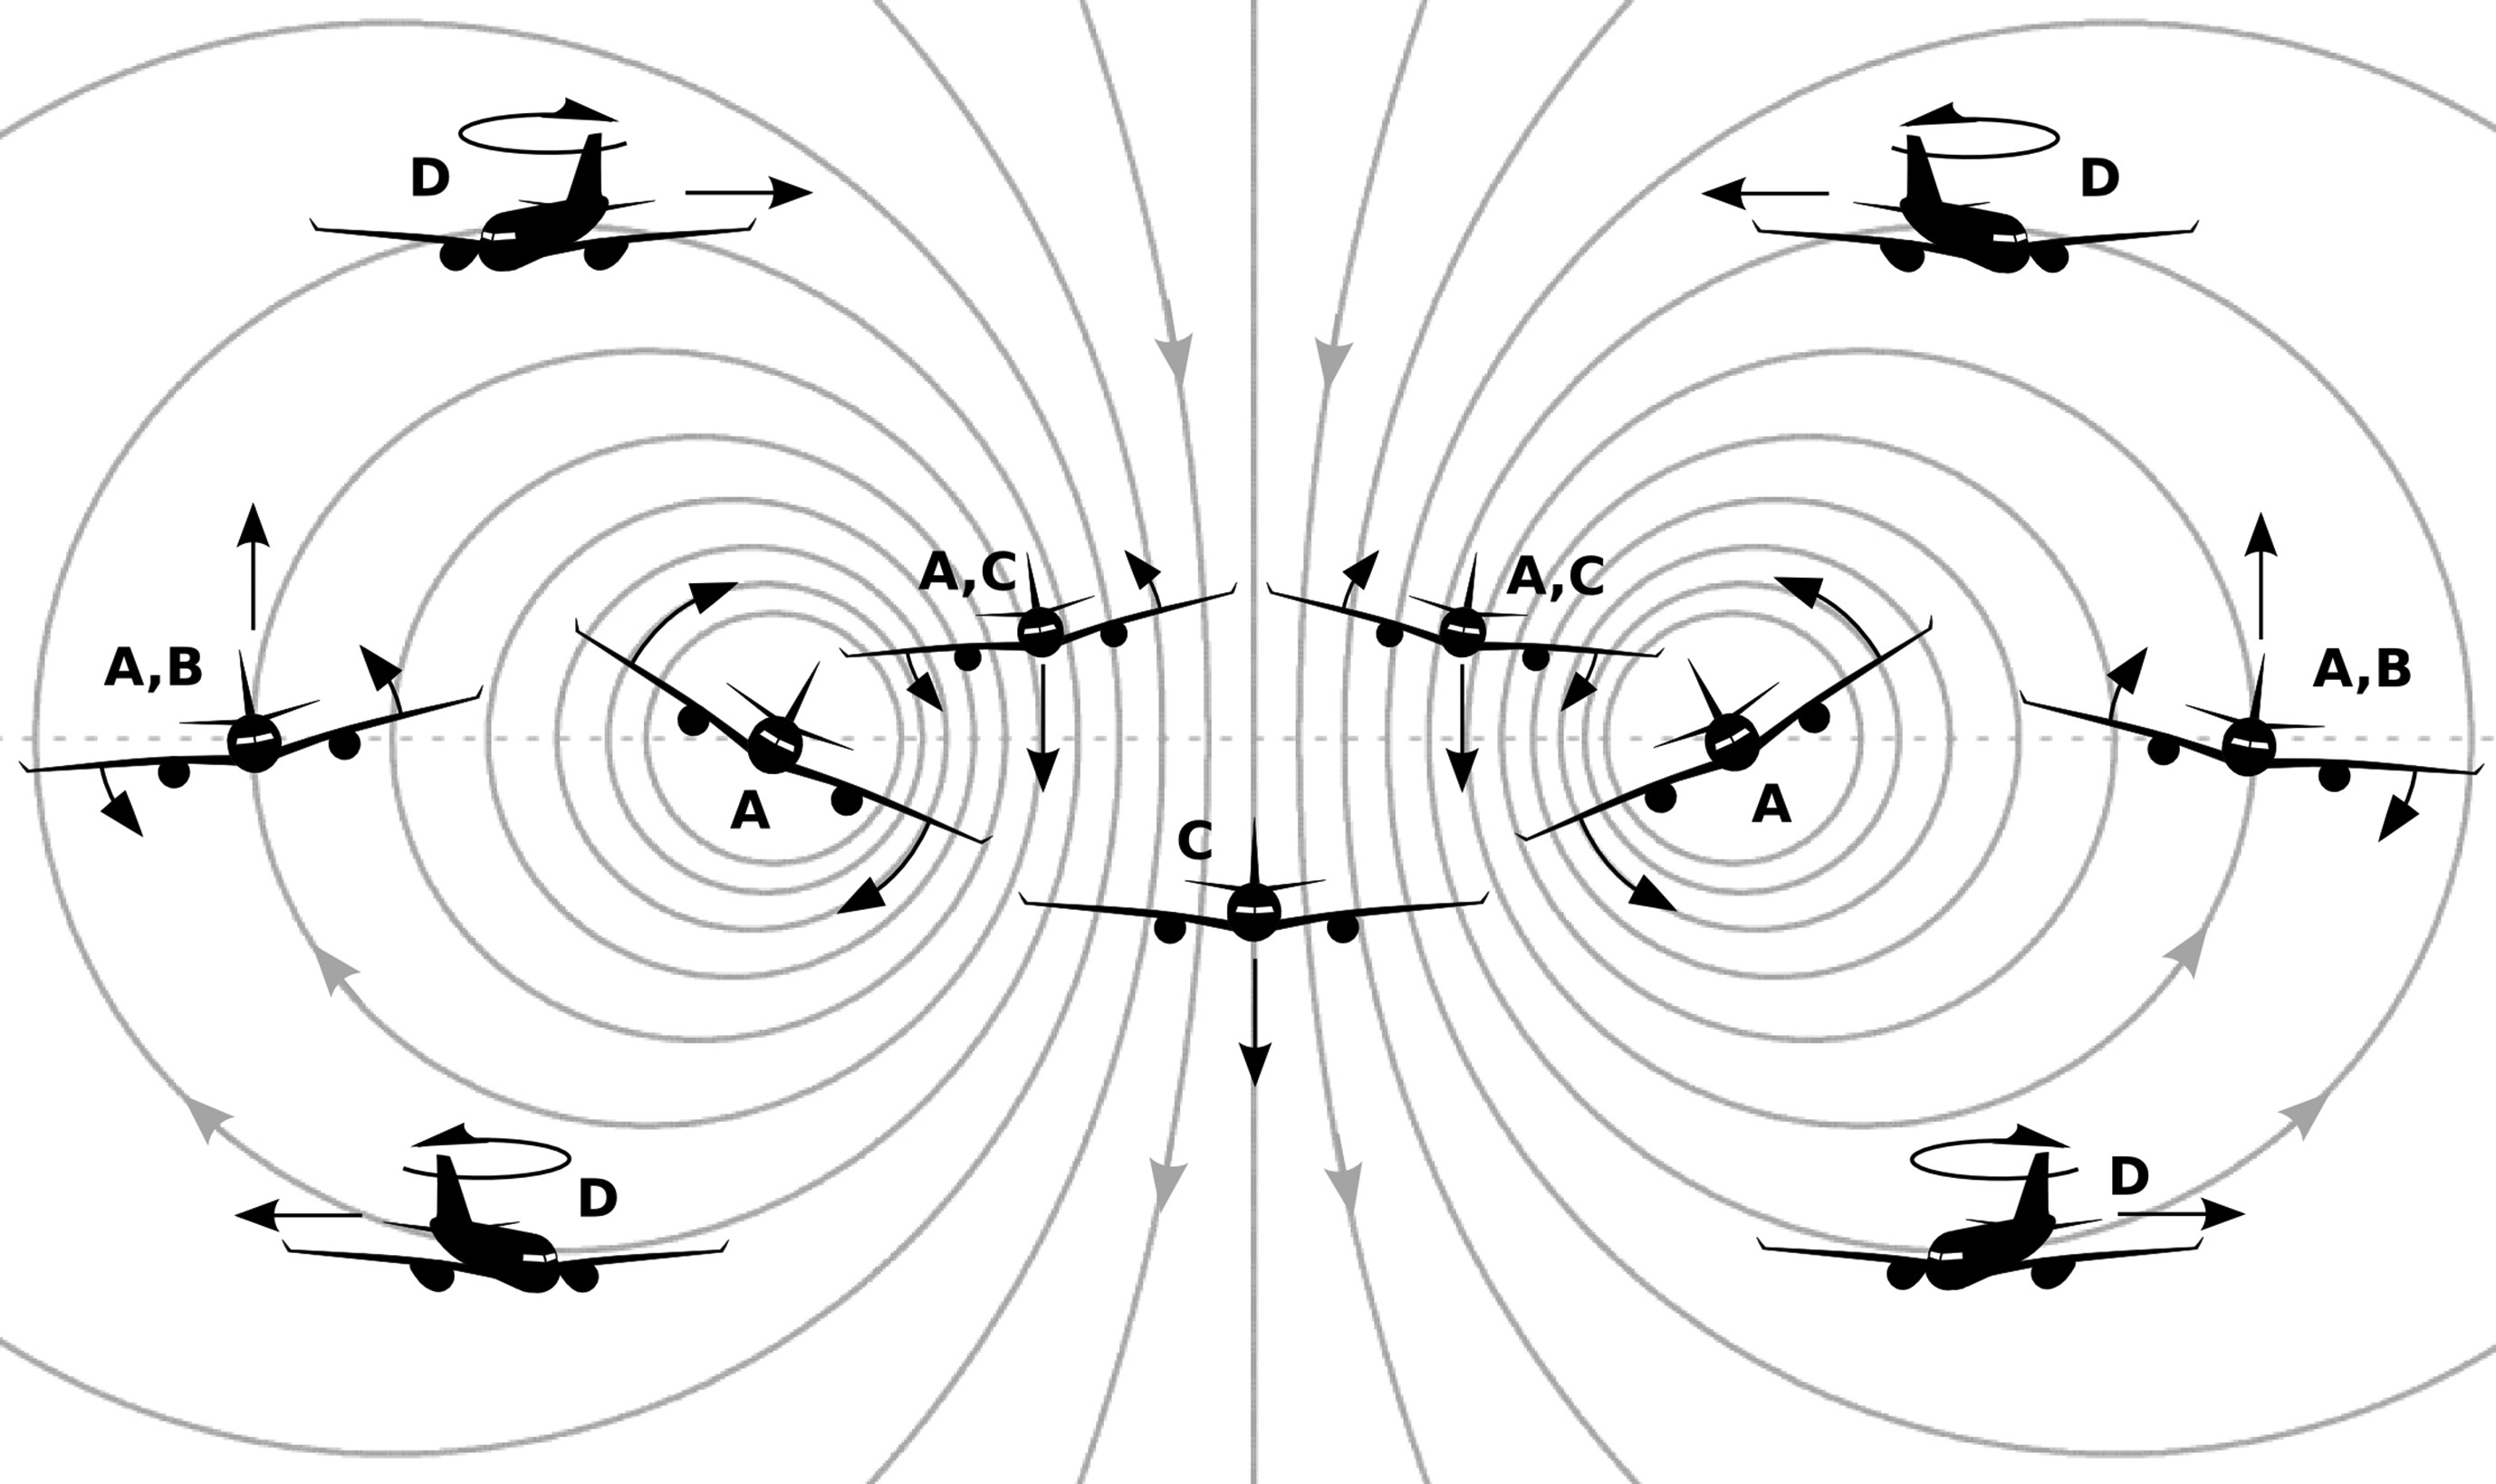
\includegraphics[width=0.8\textwidth]{graphics/reaction_in_wake.jpg}
    \caption[Wake vortex encounter]{Effect of wake vortex flow field on an aircraft. (A) induced rolling moment, (B) upward motion, (C) loss of lift  \cite[p. 33]{Hallock2018Apr}} \label{fig:vortex_encounter}
\end{figure}

Traditional separation standards, introduced in the seventies, are defined by ICAO  on the basis of certificated maximum take-off mass (MTOM) as shown in Table \ref{tab:WTC}. The prescribed categories are three (i.e.Heavy, Medium and Light). In addition for aircraft in the order of $560000$ kg ICAO provides a subcategory to the Heavy types called Super Heavy. Some states have chosen to further increase the number of categories to adapt the wake turbulence categories (WTC) to specific airport requirements. Aerodromes in the UK split the Medium and Light categories each into two subcategories (Table \ref{tab:WTC}), while the Federal Aviation Administration (FAA) places Boeing B757 into a separate category and increases the upper weight limit of the Light category. \cite{icao_wtc, uk_aeronautical_information_services_wake_2017, noauthor_recat_2018}

\begin{table}[]
    \centering
    \resizebox{1\textwidth}{!} {
    \begin{tabular}{l|c|c|c|c|c|c}
    ~    & \multicolumn{6}{c}{Category} \\ \hline
    ICAO & Super Heavy & Heavy (H) & \multicolumn{2}{c|}{Medium (M)} & \multicolumn{2}{c}{Light (L)} \\
    
    ~    & A380-800    & $ > 136000 $  & \multicolumn{2}{c|}{$ 136000-7000 $ } & \multicolumn{2}{c}{$ \leq 7000 $} \\ \hline
    
    ICAO (UK)   & ~  & Heavy (H) & Upper Medium (UM) & Lower Medium (LM) & Small (S)  & Light (L) \\
    
    ~    & A380-800    & $ > 136000 $  & $ 136000-104000 $     & $ 104000-40000 $      & $ 40000-17000 $ & $ \leq 17000 $   \\ \hline
    
    ICAO \& FAA (US)   & Super      & Heavy (H) & B757   & Large   & \multicolumn{2}{c}{Small} \\
    
    ~    & A380        & $ > 136000 $  & ~                 & $ 136000-18600 $      & \multicolumn{2}{c}{$ \leq 18600 $} \\ 
    \end{tabular}}
    \caption[ICAO wake turbulence categories based on maximum take-off mass]{ICAO wake turbulence categories based on maximum take-off mass (MTOM) in kg. \cite{icao_wtc, uk_aeronautical_information_services_wake_2017, kolos2013influence}} \label{tab:WTC}
\end{table}

The ICAO wake turbulence categories outline the worst case for each category and thus generate over-separation in many cases \cite{noauthor_recat_2018}. The separation distances for instrumental flight rules are observed for the follower aircraft and are conventionally expressed in nautical miles (NM). The separation reverts to radar separation minimum (MRS) when wake turbulence restrictions are not required. As  prescribed  by  ICAO  the  horizontal MRS is 3 NM (or a reduced separation minimum of 2.5 NM may be applied under given conditions described in ICAO Doc 4444 PANS-AM \cite{doc44444}), which translates to 79s (66s) time separation between leader and follower at approach speed of 70 m/s.


% Please add the following required packages to your document preamble:
% \usepackage{multirow}
% \usepackage{graphicx}
\begin{table}[]
\centering
\resizebox{\textwidth}{!}{%
\begin{tabular}{|c|c|c|c|c|c|}
\hline
\multicolumn{2}{|c|}{\multirow{2}{*}{ICAO WTC scheme}} & \multicolumn{4}{c|}{Follower}              \\ \cline{3-6} 
\multicolumn{2}{|c|}{}                                 & Super (A380-800) & Heavy & Medium & Light \\ \hline
\multirow{4}{*}{Leader}       & Super (A380-800)       & (*)                & 6 NM  & 7 NM   & 8 NM   \\ \cline{2-6} 
                              & Heavy                  & (*)                & 4 NM  & 5 NM   & 6 NM   \\ \cline{2-6} 
                              & Medium                 & (*)                & (*)     & (*)      & 5 NM   \\ \cline{2-6} 
                              & Light                  & (*)                & (*)     & (*)      & (*)      \\ \hline
\end{tabular}%
}
\caption[ICAO wake turbulence categories and separation minima]{ICAO wake turbulence categories and separation minima to avoid wake vortex encounter. \cite{noauthor_recat_2018, rooseleer2015recat}} \label{tab:ICAO_WTC}
\end{table}



%There is an RU logo in Figure~\ref{fig:ru-logo}.
%This logo will scale according to the width of the text on the page.

% Please add the following required packages to your document preamble:
% \usepackage{multirow}
% \usepackage{graphicx}
\begin{table}[]
\centering
\resizebox{\textwidth}{!}{%
\begin{tabular}{|c|c|c|c|c|c|c|c|}
\hline
\multicolumn{2}{|c|}{\multirow{2}{*}{RECAT-EU scheme}} & \multicolumn{6}{c|}{Follower}                   \\ \cline{3-8} 
\multicolumn{2}{|c|}{}                                 & CAT\_A & CAT-B & CAT-C & CAT-D & CAT-E & CAT-F \\ \hline
\multirow{6}{*}{Leader}             & CAT-A            & 3 NM   & 4 NM  & 5 NM  & 5 NM  & 6 NM  & 8 NM  \\ \cline{2-8} 
                                    & CAT-B            &    (*)    & 3 NM  & 4 NM  & 4 NM  & 5 NM  & 7 NM  \\ \cline{2-8} 
                                    & CAT-C            &    (*)    & (*)   & 3 NM  & 3 NM  & 4 NM  & 6 NM  \\ \cline{2-8} 
                                    & CAT-D            &    (*)    &   (*)    &    (*)   &   (*)    &   (*)    & 5 NM  \\ \cline{2-8} 
                                    & CAT-E            &    (*)    &   (*)    &   (*)    &   (*)    &   (*)    & 4 NM  \\ \cline{2-8} 
                                    & CAT-F            &    (*)    &   (*)    &    (*)   &   (*)    &   (*)    & 3 NM  \\ \hline
\end{tabular}%
}
\caption[RECAT-EU distance-based separation minima]{RECAT-EU WT distance-based separation minima on approach and departure. (*) means minimum radar separation (MRS), set at 2.5 NM, applicable as per current ICAO doc 4444 provisions \cite{doc44444, rooseleer2015recat}.}
\label{tab:RECAT-dist}
\end{table}


% Please add the following required packages to your document preamble:
% \usepackage{multirow}
% \usepackage{graphicx}
\begin{table}[]
\centering
\resizebox{\textwidth}{!}{%
\begin{tabular}{|c|c|c|c|c|c|c|c|}
\hline
\multicolumn{2}{|c|}{\multirow{2}{*}{RECAT-EU scheme}} & \multicolumn{6}{c|}{Follower}                   \\ \cline{3-8} 
\multicolumn{2}{|c|}{}                                 & CAT-A & CAT-B & CAT-C & CAT-D & CAT-E & CAT-F \\ \hline
\multirow{6}{*}{Leader}             & CAT-A            &        & 100s  & 120s  & 140s  & 160s  & 180s  \\ \cline{2-8} 
                                    & CAT-B            &        &       &       & 100s  & 120s  & 140s  \\ \cline{2-8} 
                                    & CAT-C            &        &       &       & 80s   & 100s  & 120s  \\ \cline{2-8} 
                                    & CAT-D            &        &       &       &       &       & 120s  \\ \cline{2-8} 
                                    & CAT-E            &        &       &       &       &       & 100s  \\ \cline{2-8} 
                                    & CAT-F            &        &       &       &       &       & 80s   \\ \hline
\end{tabular}%
}
\caption[RECAT-EU time-based separation minima]{RECAT-EU WT time-based separation minima on approach and departure \cite{rooseleer2015recat}}
\label{tab:RECAT-time}
\end{table}


% Please add the following required packages to your document preamble:
% \usepackage{multirow}
% \usepackage{graphicx}
\begin{table}[]
\centering
\resizebox{\textwidth}{!}{%
\begin{tabular}{|c|c|c|c|c|c|c|c|}
\hline
\multicolumn{2}{|c|}{}                                          & \multicolumn{6}{c|}{Follower}                                                                                                                                                                                                   \\ \cline{3-8} 
\multicolumn{2}{|c|}{\multirow{-2}{*}{RECAT-EU scheme}} & CAT-A                             & CAT-B                                & CAT-C                         & CAT-D                         & CAT-E                         & CAT-F                                                \\ \hline
                                                        & CAT-A & \cellcolor[HTML]{FD6864}(+0,5 NM) & \cellcolor[HTML]{67FD9A}-2 NM        & \cellcolor[HTML]{67FD9A}-1 NM & \cellcolor[HTML]{67FD9A}-2 NM & \cellcolor[HTML]{67FD9A}-1 NM &                                                      \\ \cline{2-8} 
                                                        & CAT-B &                                   & \cellcolor[HTML]{67FD9A}-1 NM        &                               & \cellcolor[HTML]{67FD9A}-1 NM &                               & \cellcolor[HTML]{FD6864}+1 NM                        \\ \cline{2-8} 
                                                        & CAT-C &                                   & \cellcolor[HTML]{67FD9A}-1 (-1,5) NM & \cellcolor[HTML]{67FD9A}-1 NM & \cellcolor[HTML]{67FD9A}-2 NM & \cellcolor[HTML]{67FD9A}-1 NM &                                                      \\ \cline{2-8} 
                                                        & CAT-D &                                   &                                      &                               &                               &                               &                                                      \\ \cline{2-8} 
                                                        & CAT-E &                                   &                                      &                               &                               &                               & \cellcolor[HTML]{67FD9A}{\color[HTML]{000000} -1 NM} \\ \cline{2-8} 
\multirow{-6}{*}{Leader}                                & CAT-F &                                   &                                      &                               &                               &                               & \cellcolor[HTML]{FD6864}(+0,5 NM)                    \\ \hline 
\end{tabular}%
}
\caption[Difference in wake separation minima on approach between reference ICAO and RECAT-EU schemes]{Difference in wake separation minima on approach between reference ICAO and RECAT-EU schemes (full proposal) \cite{rooseleer2015recat}}
\label{tab:delta_distance_wtc2recat}
\end{table}



% Please add the following required packages to your document preamble:
% \usepackage{multirow}
% \usepackage{graphicx}
\begin{table}[]
\centering
\resizebox{\textwidth}{!}{%
\begin{tabular}{|c|c|c|c|c|c|c|c|}
\hline
\multicolumn{2}{|c|}{}                                          & \multicolumn{6}{c|}{Follower}                                                                                                             \\ \cline{3-8} 
\multicolumn{2}{|c|}{\multirow{-2}{*}{RECAT-EU scheme}} & CAT-A & CAT-B                        & CAT-C & CAT-D                        & CAT-E                        & CAT-F                        \\ \hline
                                                        & CAT-A &       & \cellcolor[HTML]{67FD9A}-20s &       & \cellcolor[HTML]{67FD9A}-40s & \cellcolor[HTML]{67FD9A}-20s &                              \\ \cline{2-8} 
                                                        & CAT-B &       &                              &       & \cellcolor[HTML]{67FD9A}-20s &                              & \cellcolor[HTML]{FD6864}+20s \\ \cline{2-8} 
                                                        & CAT-C &       &                              &       & \cellcolor[HTML]{67FD9A}-40s & \cellcolor[HTML]{67FD9A}-20s &                              \\ \cline{2-8} 
                                                        & CAT-D &       &                              &       &                              &                              &                              \\ \cline{2-8} 
                                                        & CAT-E &       &                              &       &                              &                              & \cellcolor[HTML]{67FD9A}-20s \\ \cline{2-8} 
\multirow{-6}{*}{Leader}                                & CAT-F &       &                              &       &                              &                              & \cellcolor[HTML]{FD6864}+20s \\ \hline
\end{tabular}
}
\caption[Time difference between reference ICAO and RECAT-EU schemes]{Time difference in wake separation on departure between reference ICAO and RECAT-EU schemes(full proposal) \cite{rooseleer2015recat}}
\label{tab:delta_times_wtc2recat}
\end{table}


\subsection{Runway Occupancy Time}

\fxnote{describe rot in general and what factors have influence on rot, theory, models for rot, see validation for rot model paper}

\begin{figure}
    \centering
    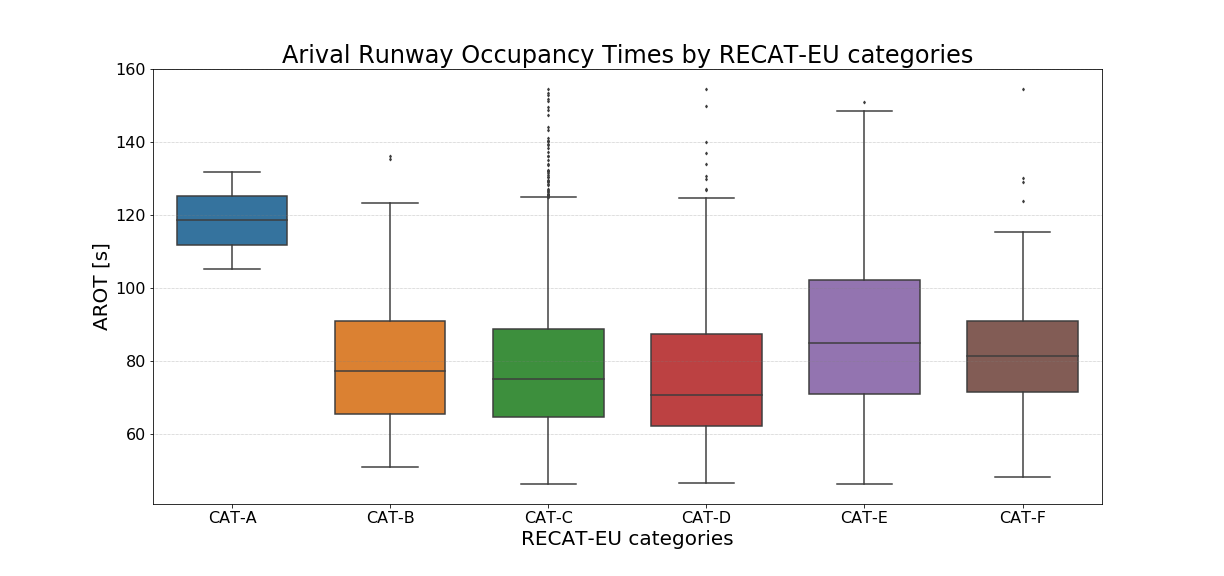
\includegraphics[width=1\textwidth]{graphics/fig_RECAT_AROTs_boxplot.png}
    \caption[AROTs boxplot for RECAT categories, all runways]{Arrival Runway Occupancy Times for the different RECAT-EU categories based on data gathered for a period of one year (since October, 2017). The box plot shows the AROTs for all runways at BIKF.}
    \label{fig:RECAT_AROTs_boxplot}
\end{figure}

The Runway Occupancy Time (ROT) is defined by Eurocontrol as the amount of time that each aircraft occupies the runway \cite{ROT_definition}. \\
This project focuses on Arrivals Runway Occupancy Time (AROT) in peak traffic hours, that is the time interval between the aircraft crossing the threshold and its tail vacating the runway \cite{AROT_definition}. The threshold is the beginning of that portion of the runway that is available for landing.
The peak traffic hours are characterised by the time intervals when the airport operates at high load. High load interval or window is at least 15 minutes in length and has four or more flights arriving or departing from Keflavik Airport. The time between flights during the high load interval is set at $\leq$4 minutes. This value is based on statistical data by Isavia in order to achieve two distinct peak hours: one in the morning and one in the afternoon. The last flight in a high load window that fulfils these requirements is not considered to be a part of the peak as its behaviour is not affected by an instantaneous next flight after it.   \fxnote{Peak hours need to be explained, Include picture}

\begin{figure}
    \centering
    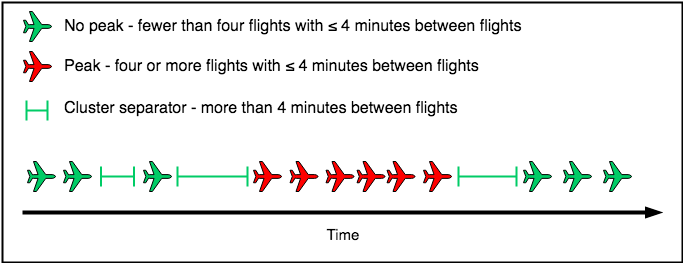
\includegraphics[width=1\textwidth]{graphics/Peak_Diagram.png}
    \caption[Rules defining a peak hour]{The rules used by Isavia to mark a high load interval as peak or not. The time separating each two aircraft in a peak cluster (red) is set as less than or equal to 4 minutes. The last red aircraft is not counted as part of the peak. Clusters are separated by time intervals larger than four minutes.}
    \label{fig:Peak_Diagram}
\end{figure}

\subsubsection{Factors affecting AROT}
\fxnote{Airfield surface condition, weather conditions, fast exits, season,  , }

% Please add the following required packages to your document preamble:
% \usepackage{graphicx}
\begin{table}[]
\centering
\resizebox{0.8\textwidth}{!}{%
\begin{tabular}{lr|r|r|r|r|r|r|r|}
\cline{3-9}
                          & \multicolumn{1}{c|}{}   & \multicolumn{7}{c|}{AROT [s]} \\ \hline
\multicolumn{1}{|l|}{RECAT-EU} & count & mean & std & min & 25\% & 50\% & 75\% & max \\ \hline
\multicolumn{1}{|l|}{CAT-A}    & 2     & 119  & 19  & 105 & 112  & 119  & 125  & 132 \\ \hline
\multicolumn{1}{|l|}{CAT-B}    & 53    & 81   & 20  & 51  & 65   & 77   & 91   & 136 \\ \hline
\multicolumn{1}{|l|}{CAT-C}    & 3449  & 78   & 17  & 41  & 65   & 75   & 89   & 155 \\ \hline
\multicolumn{1}{|l|}{CAT-D}    & 1029  & 75   & 18  & 46  & 62   & 71   & 87   & 155 \\ \hline
\multicolumn{1}{|l|}{CAT-E}    & 98    & 86   & 25  & 42  & 71   & 84   & 101  & 151 \\ \hline
\multicolumn{1}{|l|}{CAT-F}    & 50    & 83   & 23  & 43  & 69   & 81   & 91   & 155 \\ \hline
\end{tabular}%
}
\caption[AROTs for the air traffic mix by RECAT]{AROT statistics for the air traffic mix at KEF by RECAT-EU categories. The count is the number of landings in peak hours since October 2017}
\label{tab:AROT_RECAT_stats}
\end{table}


% Please add the following required packages to your document preamble:
% \usepackage{graphicx}
\begin{table}[]
\centering
\resizebox{0.8\textwidth}{!} & \multicolumn{1}{l|}{50\%} & \multicolumn{1}{l|}{75\%} & \multicolumn{1}{l|}{max} \\ \hline
\multicolumn{1}{|l|}{SUMMER} & \multicolumn{1}{r|}{3741} & 76                        & 17                       & 41                       & 63                        & 72                        & 86                        & 155                      \\ \hline
\multicolumn{1}{|l|}{WINTER} & \multicolumn{1}{r|}{940}  & 84                        & 20                       & 43                       & 69                        & 84                        & 96                        & 153                      \\ \hline
\end{tabular}%
}
\caption[AROTs for the air traffic mix by season]{AROT statistics for the air traffic mix at KEF by season. The count is the number of landings in peak hours since October 2017}
\label{my-label2}
\end{table}

% Please add the following required packages to your document preamble:
% \usepackage{graphicx}
\begin{table}[]
\centering
\resizebox{0.8\textwidth}{!} & \multicolumn{1}{l|}{50\%} & \multicolumn{1}{l|}{75\%} & \multicolumn{1}{l|}{max} \\ \hline
\multicolumn{1}{|l|}{RWY 01} & 974                        & 85                        & 22                       & 42                       & 67                        & 88                        & 99                        & 152                      \\ \hline
\multicolumn{1}{|l|}{RWY 10} & 852                        & 85                        & 11                       & 61                       & 78                        & 84                        & 91                        & 155                      \\ \hline
\multicolumn{1}{|l|}{RWY 19} & 1513                       & 67                        & 10                       & 41                       & 61                        & 66                        & 71                        & 155                      \\ \hline
\multicolumn{1}{|l|}{RWY 28} & 402                        & 68                        & 14                       & 42                       & 60                        & 66                        & 72                        & 155                      \\ \hline
\end{tabular}%
}
\caption[AROTs for the air traffic mix by runway for the summer]{AROT statistics for the air traffic mix at KEF by runway for the summer of 2018. The count is the number of landings in peak hours.}
\label{my-label3}
\end{table}


% Please add the following required packages to your document preamble:
% \usepackage{graphicx}
\begin{table}[]
\centering
\resizebox{0.8\textwidth}{!} & \multicolumn{1}{l|}{50\%} & \multicolumn{1}{l|}{75\%} & \multicolumn{1}{l|}{max} \\ \hline
\multicolumn{1}{|l|}{RWY 01} & 286                        & 88                        & 26                       & 43                       & 62                        & 90                        & 106                       & 153                      \\ \hline
\multicolumn{1}{|l|}{RWY 10} & 333                        & 93                        & 12                       & 70                       & 85                        & 91                        & 99                        & 144                      \\ \hline
\multicolumn{1}{|l|}{RWY 19} & 252                        & 72                        & 12                       & 45                       & 64                        & 70                        & 75                        & 140                      \\ \hline
\multicolumn{1}{|l|}{RWY 28} & 69                         & 73                        & 13                       & 49                       & 63                        & 72                        & 79                        & 105                      \\ \hline
\end{tabular}%
}
\caption[AROTs for the air traffic mix by runway for the winter]{AROT statistics for the air traffic mix at KEF by runway for the winter season. The count is the number of landings in peak hours since October 2017}
\label{my-label4}
\end{table}


% Please add the following required packages to your document preamble:
% \usepackage{graphicx}
% \usepackage[table,xcdraw]{xcolor}
% If you use beamer only pass "xcolor=table" option, i.e. \documentclass[xcolor=table]{beamer}
\begin{table}[]
\centering
\resizebox{0.8\textwidth}{!} & \multicolumn{1}{l|}{50\%} & \multicolumn{1}{l|}{75\%} & \multicolumn{1}{l|}{max} \\ \hline
\rowcolor[HTML]{DAE8FC} 
\multicolumn{1}{|l|}{\cellcolor[HTML]{DAE8FC}January} & 95 & 86 & 20 & 54 & 70 & 85 & 96 & 136 \\ \hline
\rowcolor[HTML]{DAE8FC} 
\multicolumn{1}{|l|}{\cellcolor[HTML]{DAE8FC}February} & 80 & 87 & 16 & 52 & 75 & 86 & 93 & 144 \\ \hline
\rowcolor[HTML]{DAE8FC} 
\multicolumn{1}{|l|}{\cellcolor[HTML]{DAE8FC}March} & 215 & 84 & 18 & 47 & 70 & 85 & 95 & 150 \\ \hline
\rowcolor[HTML]{DAE8FC} 
\multicolumn{1}{|l|}{\cellcolor[HTML]{DAE8FC}April} & 222 & 82 & 17 & 45 & 69 & 81 & 93 & 139 \\ \hline
\rowcolor[HTML]{FFFC9E} 
\multicolumn{1}{|l|}{\cellcolor[HTML]{FFFC9E}May} & 387 & 75 & 13 & 42 & 66 & 74 & 82 & 140 \\ \hline
\rowcolor[HTML]{FFFC9E} 
\multicolumn{1}{|l|}{\cellcolor[HTML]{FFFC9E}June} & 649 & 73 & 16 & 44 & 62 & 68 & 80 & 155 \\ \hline
\rowcolor[HTML]{FFFC9E} 
\multicolumn{1}{|l|}{\cellcolor[HTML]{FFFC9E}July} & 731 & 72 & 16 & 43 & 61 & 68 & 77 & 155 \\ \hline
\rowcolor[HTML]{FFFC9E} 
\multicolumn{1}{|l|}{\cellcolor[HTML]{FFFC9E}August} & 727 & 79 & 18 & 42 & 64 & 81 & 91 & 148 \\ \hline
\rowcolor[HTML]{FFFC9E} 
\multicolumn{1}{|l|}{\cellcolor[HTML]{FFFC9E}September} & 636 & 77 & 18 & 41 & 64 & 75 & 88 & 152 \\ \hline
\rowcolor[HTML]{FFFC9E} 
\multicolumn{1}{|l|}{\cellcolor[HTML]{FFFC9E}October} & 611 & 79 & 17 & 43 & 66 & 76 & 91 & 155 \\ \hline
\rowcolor[HTML]{DAE8FC} 
\multicolumn{1}{|l|}{\cellcolor[HTML]{DAE8FC}November} & 221 & 84 & 23 & 43 & 66 & 82 & 98 & 151 \\ \hline
\rowcolor[HTML]{DAE8FC} 
\multicolumn{1}{|l|}{\cellcolor[HTML]{DAE8FC}December} & 107 & 87 & 24 & 45 & 68 & 86 & 99 & 153 \\ \hline
\end{tabular}%
}
\caption[AROTs for the air traffic mix by month]{AROT statistics for the air traffic mix at KEF by month. The count is the number of landings in peak hours since October 2017}
\label{my-label5}
\end{table}





\subsection{Runway Capacity}

\fxnote{operational procedures for air traffic control at kef, }
\fxnote{equipment specifications in the tower that might influence the WTC sepatarion decision-talk to Haraldur}

subsection{AROT and LTI Objective}

\fxnote{State my hypothesis. Research objectives/research question comes in concluding part of introduction}



%%% Local Variables: 
%%% mode: latex
%%% TeX-master: "DEGREE-NAME-YEAR"
%%% End: 
